% -----------------------------------------------
% Template for SMC 2009
%     smc2009.sty -> style file
% Last modified by Fabien Gouyon (smc2009@inescporto.pt)
% Modified by Juan P. Bello (ismir2008-papers@ismir.net)
% By Rainer Typke (ismir07.rainer@safersignup.com)
% Based on the 2004 template by Eloi Batlle.
% -----------------------------------------------

\documentclass{article}
\usepackage{smc2009,amsmath}
% To use when using pdflatex
\usepackage{graphicx}
\usepackage{url}
% To use when using latex, dvips and ps2pdf
% \usepackage[dvips]{graphicx}

% Title.
% ------
\title{Paper Template for SMC 2009}

% IMPORTANT NOTICE:
% Reviews are double-blind
% Authors will not be informed of who reviews their papers, and author names will be concealed from the reviewers 
% Please avoid evident self references in the text

% Authors' names must be omitted from title page (or listed as �name(s) omitted for submission�)


% Single address
% To use with only one author or several with the same address
% ---------------
%\oneauthor
%   {Author} {School \\ Email}

% Two addresses
 %--------------
\twoauthors
  {First author} {School \\ Email}
  {Second author} {Company \\ Email}

% Three addresses
% --------------
%\threeauthors
%  {First author} {School \\ Email}
%  {Second author} {Company \\ Email}
%  {Third author} {Company \\ Email}


\begin{document}
%
\maketitle
%

\permission

\begin{abstract}
The abstract should be placed at the top left column and should contain
about 150-200 words.
\end{abstract}

\section{Introduction}\label{sec:introduction}

This template includes all the information about formatting manuscripts for the SMC 2009. Please follow these 
guidelines to give the final proceedings a uniform look. If you have any questions, please contact the conference Programme Chairs.

This template (in Word and Latex formats) can be downloaded from the SMC 2009 web site 
(\url{http://smc2009.smcnetwork.org/}). (Some users may recognize that this template is an adaptation of the ISMIR template.)

%\section{Pdflatex versus Latex/dvips}
%You can prepare a PDF file in two ways: either directly with pdflatex (using
%Template.tex) or with latex, dvips, and ps2pdf (using Template\_ps.tex). The
%latter method allows you to include Postscript images, while the former
%works nicely with PNG or PDF images, just to name two examples.

\section{Page Size}\label{sec:page_size}

The proceedings will be printed on letter-size paper (21.6 x 27.9 cm or
8.5" x 11").
All material on each page should fit within a rectangle of 7" x 9" (17.78~cm x 22.86~cm), 
centered on the page, beginning 1'' (2.54~cm)
from the top of the page and ending with 1'' (2.54~cm) from the
bottom. The left and right margins should be 0.75'' (1.9~cm).
The text should be in two 3.3" (8.4~cm) columns with a 0.4'' (1~cm) gutter.
All {\it text} must be in a two-column format. Text must be
{\it \textbf{fully justified}}.


\section{Typeset Text}\label{sec:typeset_text}

\subsection{Normal or Body Text}\label{subsec:body}

Please use a 10pt (point) Times font, or other Roman font with serifs, as close as possible in appearance to Times. 
Please use sans-serif or non-proportional fonts only for special purposes, such as distinguishing source code text.

The first paragraph in each section should not be indented, but all other paragraphs should be.

\subsection{Title and Authors}

The title is 14pt Times, bold, caps, upper case, centered. Authors' names are centered. 
The lead author's name is to be listed first (left-most), and the co-authors' names after. If the addresses for all 
authors are the same, include the address only once, centered. If the authors have different addresses, 
put the addresses, evenly spaced, under each authors' name.

Reviews are double-blind. {\it \textbf{Author information should be removed from this page in initial submissions}}, 
and only added later by the authors when sending camera-ready versions.

\subsection{Page Numbering, Headers and Footers}

Do not include headers, footers or page numbers in your submission.
These will be added when the publications are assembled.

\section{First Level Headings}

First level headings are in Times 10pt bold, centered with 1 line
of space above the section head, and 1/2 space below it.  For a section
header immediately followed by a subsection header, the space should be merged.

\subsection{Second Level Headings}

Second level headings are in Times 10pt bold, flush left, with 1 line of
space above the section head, and 1/2 space below it. The first letter of
each significant word is capitalised.

\subsubsection{Third and Further Level Headings}

Third level headings are in Times 10pt italic, flush left, with 1/2 line
of space above the section head, and 1/2 space below it. The first letter
of each significant word is capitalised.

Using more than three levels of headings is highly discouraged.

\section{Footnotes and Figures}

\subsection{Footnotes}

Indicate footnotes with a number in the text.\footnote{This a footnote}
Use 8pt type for footnotes. Place the footnotes at the bottom of the page
on which they appear. Precede the footnote with a 0.5pt horizontal rule.

\subsection{Figures, Tables and Captions}

All artwork must be centered, neat, clean, and legible. All lines should
be very dark for purposes of reproduction and art work should not be hand-drawn.
The proceedings is not in color, and therefore all figures must make
sense in black-and-white form.
Figure and table numbers and captions always appear below the figure. Leave 1
line space between the figure or table and the caption. Each figure or table
is numbered consecutively. Captions should be Times 10pt.
Place tables/figures in text as close to the reference as possible.
References to figures and tables should be capitalised, for example:
see Figure \ref{fig:example} and Table \ref{tab:example}.
Figures and tables may extend across both columns to a maximum
width of 7'' (17.78~cm).

\begin{table}
\begin{center}
\begin{tabular}{|l|l|}
\hline
String value & Numeric value \\
\hline
hello SMC  & 1073 \\
\hline
\end{tabular}
\end{center}
\caption{Table captions should be placed below the table}
\label{tab:example}
\end{table}

\begin{figure}
\centerline{\framebox{
% To use when using pdflatex
	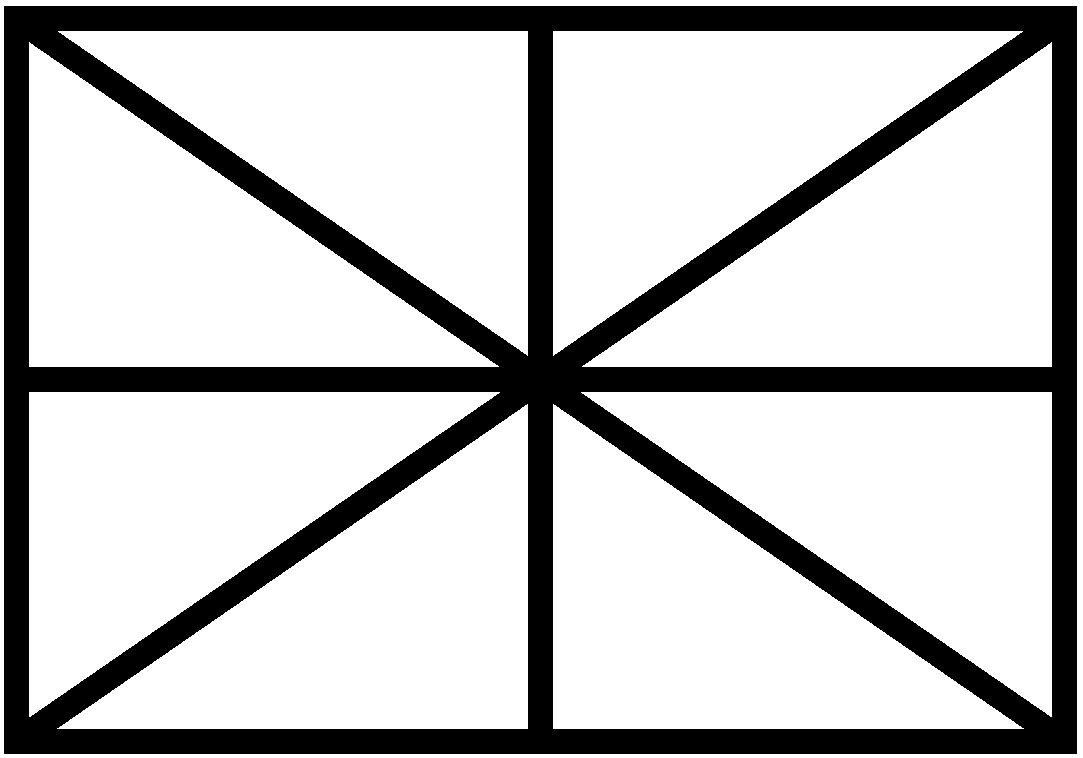
\includegraphics[width=\columnwidth]{figure.png}}}
	% To use when using latex, dvips and ps2pdf
% 	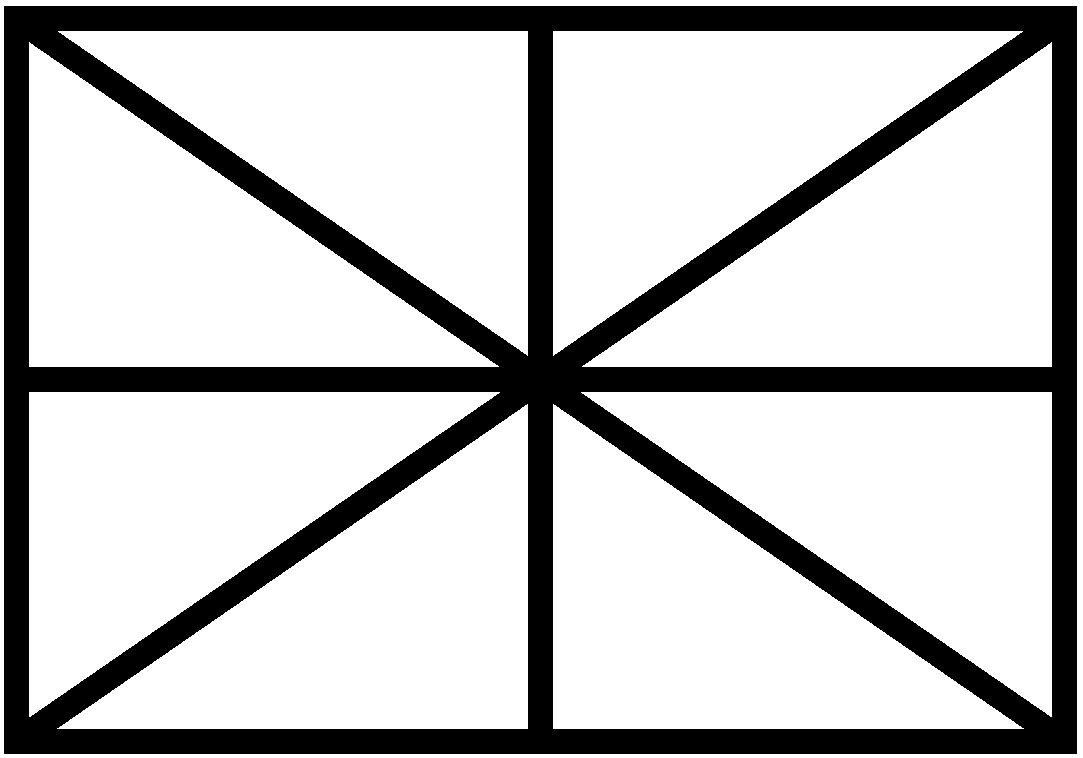
\includegraphics[width=\columnwidth]{figure.eps}}}
\caption{Figure captions should be placed below the figure}
\label{fig:example}
\end{figure}

\section{Equations}

Equations should be placed on separated lines and numbered.
The number should be on the right side, in parentheses.

\begin{equation}
E=mc^{2}
\end{equation}

\section{Citations}

All bibliographical references should be listed at the
end, inside a section named ``REFERENCES''.
All references listed should be cited in the text.
When refering to a document, type the number in
square brackets~\cite{Author:00}.

\begin{thebibliography}{citations}

\bibitem {Author:00} Author, E.
``The title of the conference paper'',
{\it Proceedings of the 5th Sound and Music Computing Conference}, 
Berlin, Germany, 2008.

\bibitem{Someone:02} Someone, A.
{\it  Title of the book}.
Editorial Acme, Barcelona, 2004.

\end{thebibliography}

\end{document}
